\documentclass[a4paper]{report}
\usepackage[T1]{fontenc}
\usepackage[portuguese]{babel}
\usepackage{url}
\usepackage{cite}
\usepackage[T1]{fontenc}
\usepackage[utf8]{inputenc} 
\usepackage[printonlyused]{acronym}
\usepackage{hyperref} 
\usepackage{totcount}
\usepackage{blindtext}
\usepackage{color,graphicx}
\usepackage{float}

\definecolor{blue}{rgb}{0,0,0.5}
\definecolor{red}{rgb}{0.6,0,0}
\definecolor{green}{rgb}{0,0.5,0}
\definecolor{gray}{rgb}{0.5,0.5,0.5}

\DeclareFixedFont{\ttb}{T1}{txtt}{bx}{n}{12}
\DeclareFixedFont{\ttm}{T1}{txtt}{m}{n}{12} 

\regtotcounter{chapter}

\begin{document}

\def\titulo{PROJETO 2 (Proj2)}
\def\data{Junho 2018}
\def\autores{António Macedo, João Oliveira, João Tomás Simões, Martim Neves (Grupo 3)}
\def\autorescontactos{(66425) amrm@ua.pt, (87874) joaomsoliveira@ua.pt}
\def\autorescontacto{(88930) jtsimoes@ua.pt, (88904) martimfneves@ua.pt}
\def\versao{MIECT}
\def\departamento{Laboratórios de Informática (Turma 4)}
\def\empresa{Universidade de Aveiro}
\def\logotipo{ua.pdf}

\begin{titlepage}

\begin{center}

\vspace*{50mm}

{\Huge \titulo}\\ 

\vspace{10mm}

{\Large \empresa}\\

\vspace{10mm}

{\LARGE \autores}\\ 

\vspace{30mm}

\begin{figure}[h]
\center
\includegraphics{\logotipo}
\end{figure}

\vspace{30mm}
\end{center}

\begin{flushright}
\versao
\end{flushright}
\end{titlepage}

\title{
{\Huge\textbf{\titulo}}\\
\vspace{3mm}
{\Large \departamento\\ \empresa}
}

\author{
\autores \\
\autorescontactos \\
\autorescontacto
}

\date{\data}

\maketitle

\pagenumbering{roman}

\renewcommand{\abstractname}{Agradecimentos}
\begin{abstract}

Deixamos aqui um agradecimento ao professor João Paulo Barraca e ao professor Vitor Cunha pela enorme disponibilidade de ambos em ajudarem-nos neste nosso trabalho e pelas dicas valiosas que nos recomendaram a implementar para que o nosso código ficasse ainda melhor. 

Sem a vossa ajuda não seria possível a conclusão deste projeto. 
Mais uma vez, obrigado por nos serem tão prestáveis e por esclarecerem as nossas inúmeras dúvidas. Esperamos que esta nossa aplicação esteja do vosso agrado.

\end{abstract}

\tableofcontents  

\clearpage
\pagenumbering{arabic}

\chapter{Introdução}
\label{chap.introducao}
\paragraph{}No âmbito da unidade curricular de \ac{labi}, foi-nos proposto a realização de um \ac{p2} cujo objetivo foi a criação de um sistema que permite que sejam geradas músicas através de trechos de outras músicas. 

\paragraph{}Para isso foi feito uso de uma 	interface web, através da qual é feito todo o contacto com o utilizador. Além disso, foi também utilizada uma \ac{ap} que permite o fluxo de informação entre as várias páginas e os seus múltiplos constituintes. De seguida foi utilizada uma \ac{bd} para armazenar todas as informações relativas a cada música. Por fim foi criado um gerador de músicas que, passando-lhe uma pauta como argumento, gera a música contida nessa pauta. 

\paragraph{}Assim, neste documento, irá perceber-se qual foi a nossa maneira de pensar e de implentar o código, assim como explicá-lo e testá-lo. Para isso, este documento está dividido em \total{chapter} capítulos.

\paragraph{}Depois desta introdução virá o \autoref{chap.explicacao}, onde apresentamos o nosso programa divido em blocos de código (funções) e em baixo de cada um explicamos o nosso pensamento enquanto o implementávamos e explicamos também qual a sua função.
No \autoref{chap.testes} são apresentados alguns testes feitos por experimentação que demonstram a funcionalidade do programa.
De seguida, no \autoref{chap.discussao}, serão discutidas as dificuldades na elaboração do código, bem como os bugs conhecidos e outros tópicos considerados relevantes.
Finalmente, no \autoref{chap.conclusao} são apresentadas as conclusões deste trabalho.

\chapter{Explicação dos vários blocos de código (funções)}
\label{chap.explicacao}

\section{\textit{Interface Web}}

\paragraph{}Para a criação da interface web foi necessário criar três páginas, cada uma delas construída com \ac{html}, \ac{js} e \ac{css} que, como já foi referido, vão ser o único meio de contacto entre o utilizador e o sistema.
\paragraph{}Na primeira página são listadas todas as músicas por ordem alfabética crescente, bem como um reprodutor de áudio que permite que todas as músicas sejam reproduzidas. Existem ainda botões de voto (positivo ou negativo), através dos quais os vários utilizadores podem expressar a sua opinião relativamente a cada música.

\begin{figure}[H]
\center
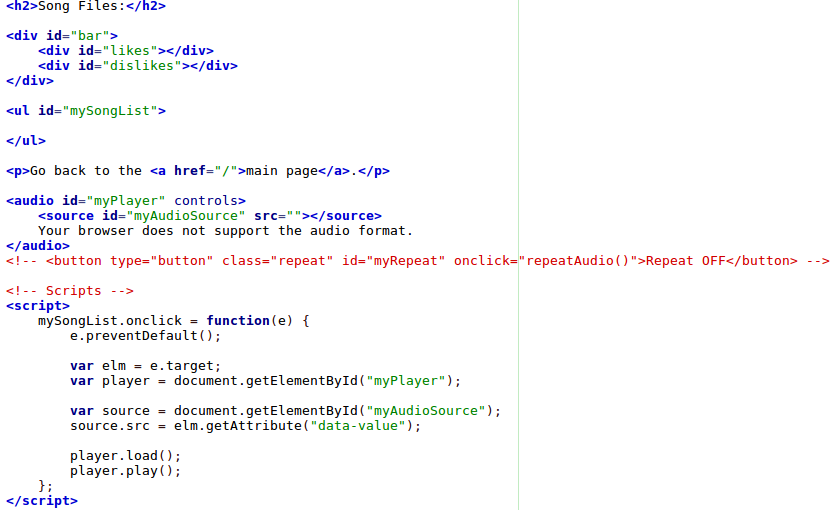
\includegraphics[width=9cm]{imagens/page1}
\caption{Página 1}
\end{figure}
\paragraph{}Na primeira página é criado o reprodutor de áudio e é chamada uma função desenvolvida em \textit{\textbf{Python}} que vai listar todas as músicas existentes.

\begin{figure}[H]
\center
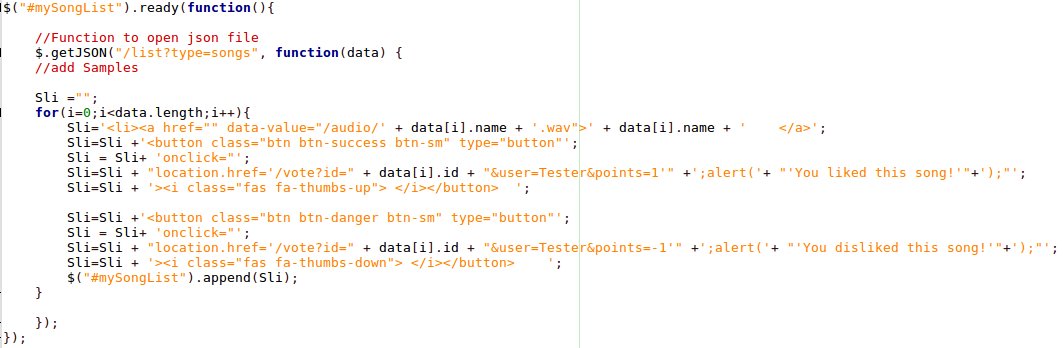
\includegraphics[height=5cm] {imagens/page1_function}
\caption{Função para listar músicas}
\end{figure}
\paragraph{}Esta função abre o ficheiro \ac{json} e cria uma \textit{\textbf{string}} à qual acrescenta o nome de todas as músicas existentes, fazendo uso de um ciclo \textit{\textbf{for}} para percorrer o ficheiro. Além disso são também criados dois botões para o utilizador poder votar positiva ou negativamente na musica.

\newpage

\paragraph{}Na segunda página são listados todos os trechos existentes, os quais podem ser utilizados mais tarde para a criação de músicas. Tal como na primeira página, existe também um reprodutor para que seja possível a reprodução de todas as músicas. Além disso, existe um botão que permite que o utilizador envie um trecho seu para mais tarde poder ser utilizado na composição de músicas.

\begin{figure}[H]
\center
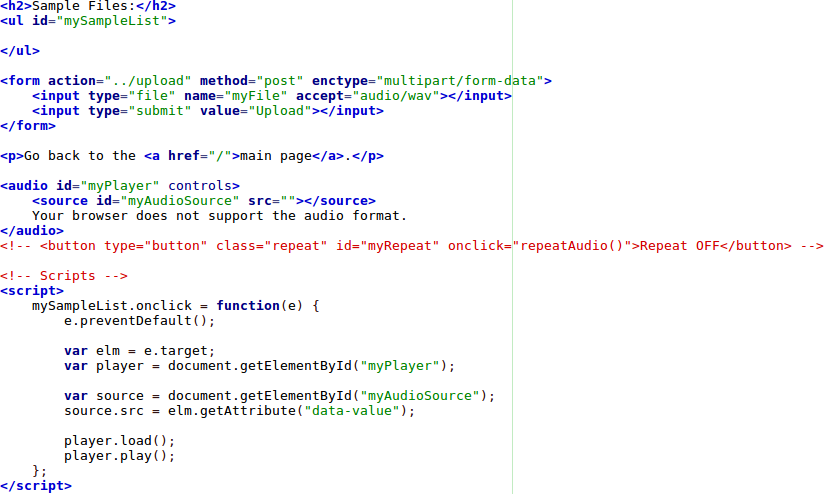
\includegraphics[width=9cm] {imagens/page2}
\caption{Página 2}
\end{figure}
\paragraph{}Na página 2 é criado um botão que permite que o utilizador envie um \textit{\textbf{sample}} seu para usar na composição de músicas. Para além disso é chamada outra função desenvolvida em \textit{\textbf{Python}} que, tal como a função da página 1, lista o conteúdo do fiheiro \ac{json}, só que desta vez retorna uma lista de \textit{\textbf{samples}}.

\begin{figure}[H]
\center
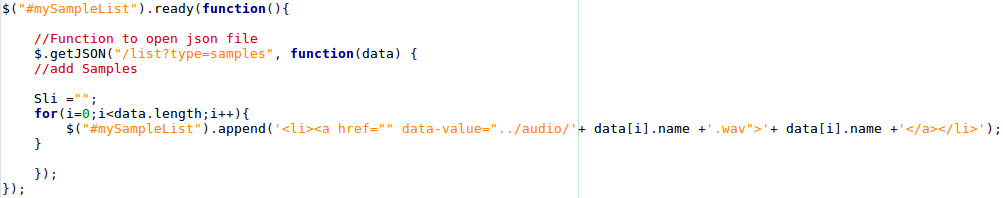
\includegraphics[height=3cm] {imagens/page2_function}
\caption{Função para listar \textit{\textbf{samples}}}
\end{figure}
\paragraph{}Tal como referido anteriormente, esta função faz o mesmo que a função da página 1 (abrir o ficheiro \ac{json} e criar uma \textit{\textbf{string}} à qual vão sendo adicionados os vários \textit{\textbf{samples}} à medida que se percorre o ficheiro).

\newpage

\paragraph{}Na terceira página existe uma tabela que permite que o utilizador escolha um trecho e um efeito a aplicar a esse trecho. Ao longo de vinte tempos, o utilizador vai escolher quando quer que cada trecho seja utilizado e, carregando num botão, será enviada para a \ac{ap} uma pauta correspondente às escolhas do utilizador, pauta essa que será processada e transformada numa música.

\begin{figure}[H]
\center
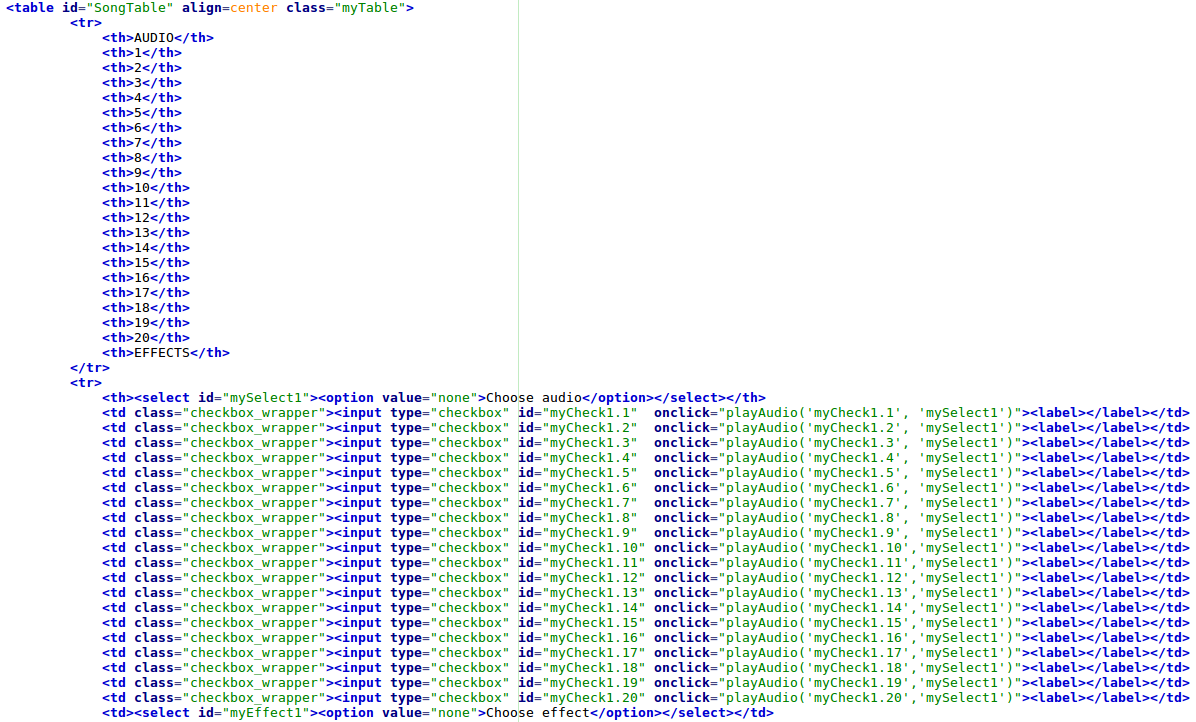
\includegraphics[width=11cm] {imagens/page3_1}
\caption{Página 3}
\end{figure}
\paragraph{}Na terceira e última página é criada uma tabela com várias \textit{\textbf{checkboxes}}, tabela essa que vai servir para o utilizador definir que trechos quer que toquem, em que momento e com que efeito, gerando assim uma pauta. Nesta página existem também um botão \textit{\textbf{rec}}, para guardar a pauta gerada e criar a música, e um botão \textit{\textbf{reset}}, que deseleciona todas as \textit{\textbf{checkboxes}}, trechos e efeitos, tal como mostrado na figura seguinte.
\begin{figure}[H]
\center
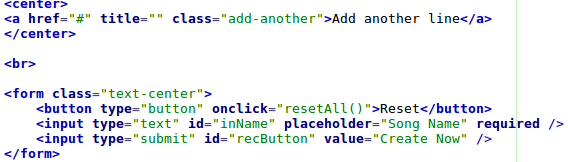
\includegraphics[width=9cm] {imagens/page3_2}
\caption{Página 3}
\end{figure}

\newpage

\paragraph{}Existe ainda uma opção para adicionar mais uma linha, caso o utilizador queira uma música que use mais \textit{\textbf{samples}}. Para isso foi desenvolvida em \ac{js} a seguinte função:
\begin{figure}[H]
\center
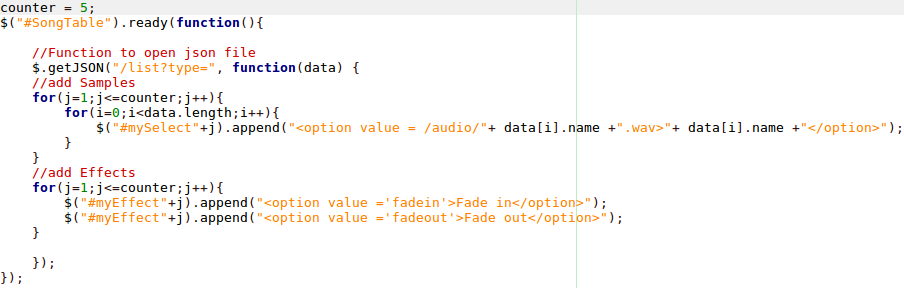
\includegraphics[height=5cm] {imagens/page3_function}
\caption{Função para acrescentar linha}
\end{figure}
\paragraph{}Esta função faz uso de um ciclo \textit{\textbf{for}} para criar uma nova entrada e adicionar todos os trechos e efeitos possíveis de serem utilizados.

\begin{figure}[H]
\center
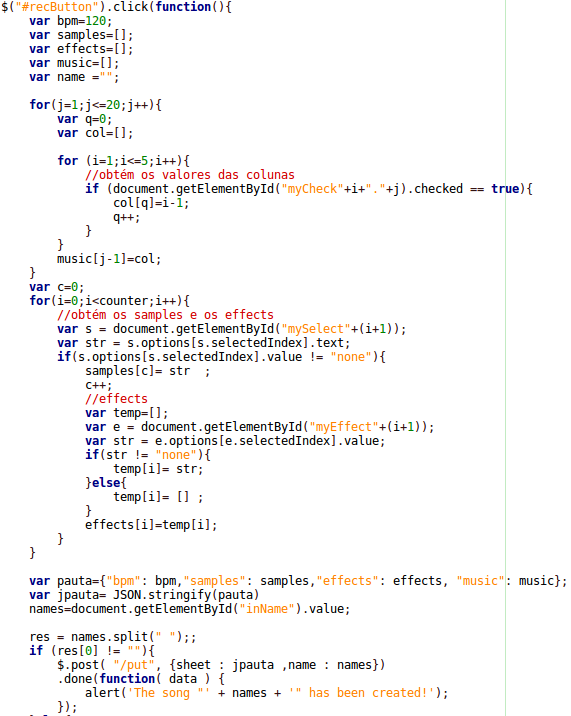
\includegraphics{imagens/page3_recbutton}
\caption{Botão para gerar música}
\end{figure}
\paragraph{}O botão \textit{\textbf{rec}} é descrito pela função acima apresentada. Através de vários ciclos \textit{\textbf{for}} é possível saber quais os \textit{\textbf{samples}} e efeitos selecionados e os tempos em que cada \textit{\textbf{sample}} é reproduzido. Esses elementos constituem a pauta, pauta essa que é depois convertida para \ac{json}.Analisando o nome dado à música que está prestes a ser criada, se o nome for válido, a música é criada. Caso contrário, deverá ser introduzido um novo nome.

\newpage

\section{\textit{Aplicação Web}}

\paragraph{}Nesta secção foi desenvolvida a \ac{ap}. A \ac{ap} consiste essencialmente num programa em \textit{\textbf{Python}} que serve conteúdos estáticos. É através da \ac{ap} que são executadas todas as funcionalidades deste projeto, nomeadamente:
\begin{enumerate}
   \item \textbf{/list?type=songs}: devolve um objeto \ac{json} com todas as músicas já criadas e a respetiva informação de cada música, como por exemplo data de criação, nome, identificador, etc. 
   \item \textbf{/list?type=samples}: muito semelhante ao anterior no entanto, em vez de devolver um objeto \ac{json} com todas as músicas e as suas caraterísticas, o objeto \ac{json} é referente aos trechos existentes e às suas caraterísticas.
   \item \textbf{/get?id=identificador}: permite identificar uma música ou um trecho através do seu identificador.
   \item \textbf{/put}: permite o envio de uma pauta, juntamente com o nome da música, para que seja criada uma nova música apartir da pauta.
   \item \textbf{/vote?id=identificador\&user=uid\&points=1}: permite que um determinado utilizador (autenticado pelo próprio XCOA ao iniciar a \ac{ap}) vote numa determinada música, sendo que o voto pode ser positivo ou negativo.
\end{enumerate}

\paragraph{}A declaração das funções são muito semelhantes entre si e o código interno\cite{guiao} das mesmas também é facilmente compreensível, mas mesmo assim vamos explicar algum mais complexo nos capítulos seguintes.

\newpage

\section{\textit{Persistência}}

\paragraph{}Nesta secção do trabalho o objetivo foi a criação de uma \ac{bd} relacional que contivesse toda a informação acerca dos trechos e músicas existentes, sendo que apenas a informação se encontra na \ac{bd} pois os ficheiros \ac{wave} que contêm os trechos e as músicas estão guardados no sistema de ficheiros da \ac{ap}. Além disso foi também necessária a criação de métodos para ler e escrever informação na \ac{bd}.

\begin{figure}[H]
\center
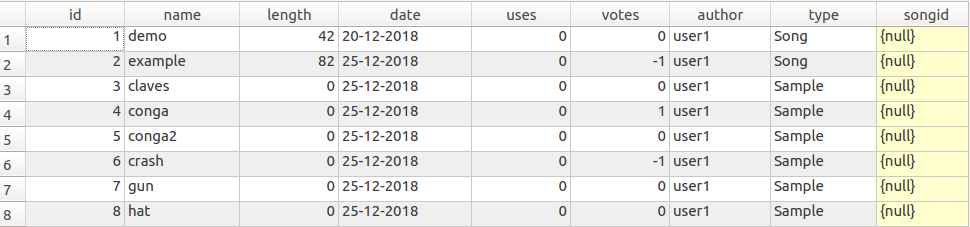
\includegraphics[width=13cm] {imagens/database}
\caption{Tabela com informação dos \textit{\textbf{samples}}}
\end{figure}

\begin{figure}[H]
\center
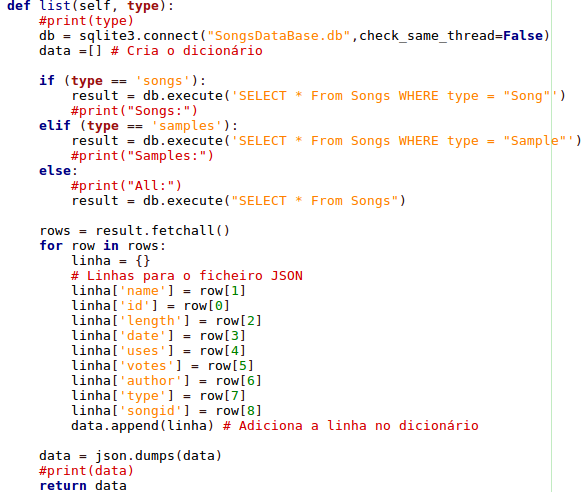
\includegraphics[height=7cm] {imagens/leiturabd}
\caption{Exemplo de leitura de dados da \ac{bd}}
\end{figure}
\paragraph{}O código acima mostra como se podem ler os dados contidos na \ac{bd}. Primeiro é estabelecida ligação à \ac{bd}. Depois, selecionando apenas as músicas, \textit{\textbf{samples}} ou todo o conteúdo existente na \ac{bd}, o resultado vai ser impresso. Após a impressão dos resultados, todas as informações correspondentes aos dados impressos são passadas para o ficheiro \ac{json}.

\begin{figure}[H]
\center
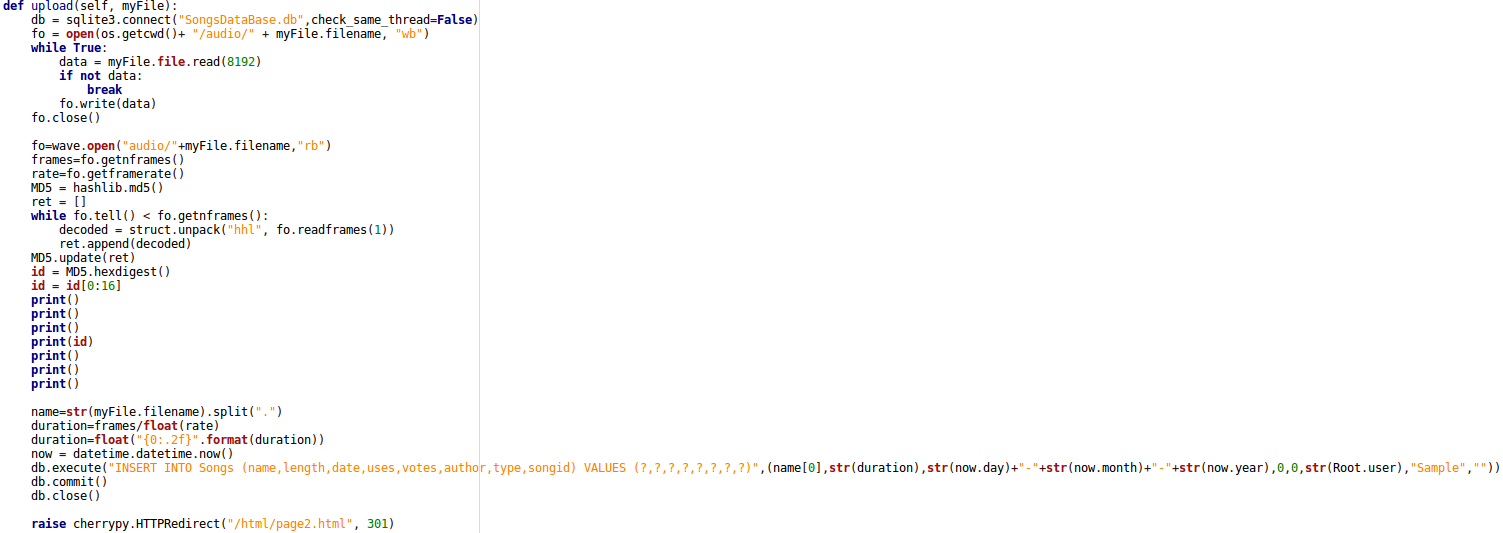
\includegraphics[width=16.5cm] {imagens/escritabd}
\caption{Exemplo de escrita de dados na \ac{bd}}
\end{figure}
\paragraph{}Neste exemplo de escrita de dados na \ac{bd}, tal como no exemplo acima, a primeira coisa a fazer é estebelecer ligação à \ac{bd}. De seguida é mostrado o código para o botão de \textit{\textbf{upload}}. É criado um \textit{\textbf{id}} baseado na conteúdo da música e de seguida as informações referentes a essa música são escritas na \ac{bd}. 

\newpage

\section{\textit{Gerador de Músicas}}

\paragraph{}Nesta parte do projeto foi desenvolvido o gerador de músicas. Este gerador permite que o utilizador lhe mande uma pauta com dados de uma música e o gerador vai transformar essa pauta em música, de acordo com os dados nela presentes. Caso a geração seja bem sucedida, o ficheiro \ac{wave} vai ser guardado no sistema de ficheiros e a informação relativa à música gerada será armazenada na \ac{bd}, sendo que o identificador da música é gerado de acordo com o seu conteúdo.

\begin{figure}[H]
\center
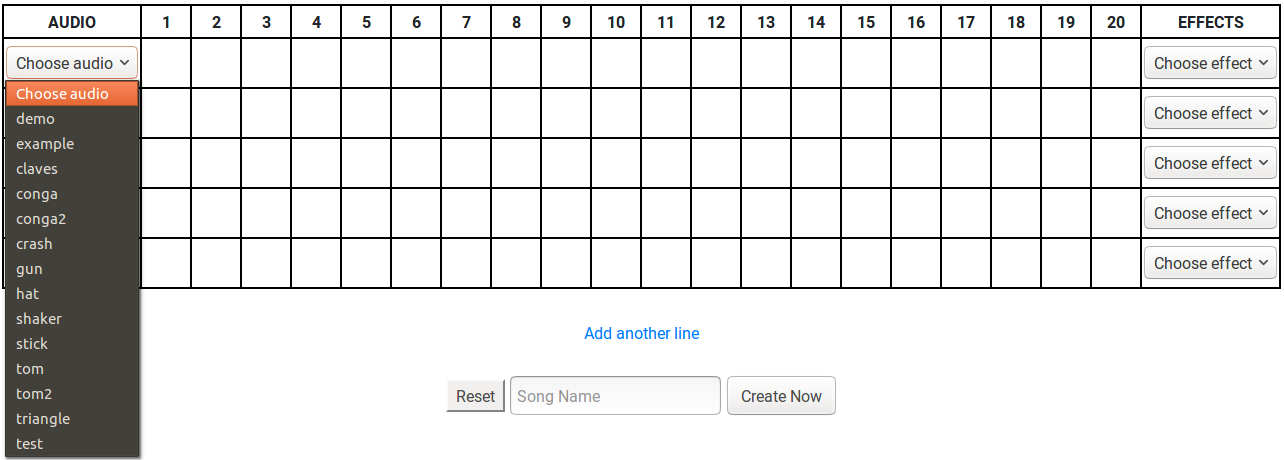
\includegraphics [width=13cm] {imagens/interface_page3}
\caption{Interface do Gerador de Músicas}
\end{figure}

\begin{figure}[H]
\center
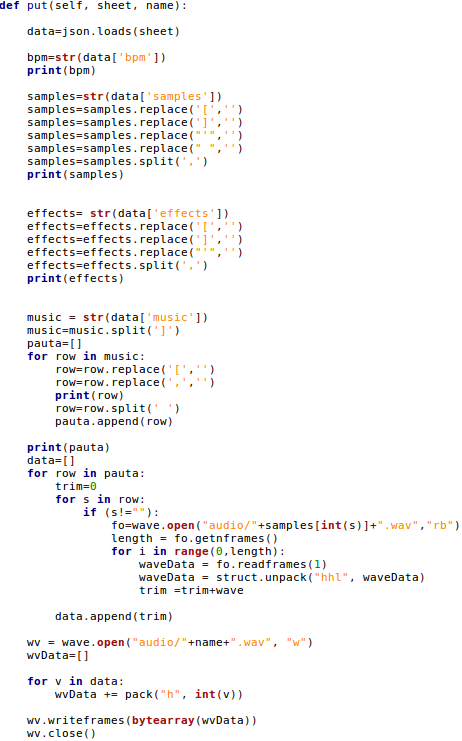
\includegraphics[height=12cm] {imagens/criar_musica}
\caption{Código para criar música a partir da pauta}
\end{figure}
\paragraph{}Neste excerto de código é mostrado o processo de criação de músicas através da pauta. São selecionados todos os trechos e efeitos usados na criação e são adicionados no mesmo ficheiro \ac{wave} nos tempos selecionados pelo utilizador.

\newpage

\chapter{Testes}
\label{chap.testes}

\paragraph{}Ao longo da escrita do nosso código fomos implementando e ao mesmo tempo testando algumas funções e verificámos apenas um bug em todo o nosso código.

\paragraph{}O bug existe no que toca aos votos. Teoricamente, o utilizador só podia dar um \textit{like} ou um \textit{dislike}. Quando o utilizador clicava no botão de \textit{like}, o mesmo botão ficava com o atributo \textit{disable} e o utilizador apenas poderia clicar no botão \textit{dislike} e vice-versa. Ao fazer alguns testes, verificámos que isso não acontece. E, por falta de tempo, não conseguimos corrigir este erro mas ponderámos ainda um pouco e chegámos à conclusão que muito provavelmente está relacionado com a \ac{bd} e não com o \ac{js} nem com o \ac{html}.

\paragraph{}É de notar também que o tempo não permitiu adicionar efeitos às músicas no criador de sons (página 3). O dicionário \ac{json} ainda foi iniciado mas não conseguimos concluir o código Python para os aplicar às músicas geradas pela página 3. Não tendo tempo para concluir os módulos obrigatórios, certamente que não houve tempo para realizar também o módulo bónus intitulado "Gerador de Imagens", embora com muita pena nossa visto que não parecia complicado.

\paragraph{}Outro pequeno detalhe que verificámos foi que se o utilizador selecionasse uma música muito longa na tabela de criar sons (página 3), ela ficaria a tocar até ao fim e caso o utilizador selecionasse mais sons, tornava-se irritante e muito barulhento. A solução que encontrámos foi colocar todas as músicas a tocar apenas por 5 segundos seguido de um \textit{fade out} quando o utilizador marca a \textit{checkbox} correspondente.

\paragraph{}De resto, a aplicação está a executar normalmente e como pedido no guião, não havendo mais erros graves a notar.

\newpage

\chapter{Discussão}
\label{chap.discussao}

\paragraph{}Tivemos algumas dificuldades nomeadamente aquando do envio da \ac{ap} para o XCOA, visto que alterou imensos caminhos que tivemos de retificar posteriormente. Entraram em conflito também alguns problemas na base de dados mas foi tudo corrigido, mais uma vez graças à ajuda e dicas dos docentes.

\paragraph{}Uma coisa que foi notada por todos os membros deste grupo foi que o projeto era um pouco extenso para o tempo dado. Como se verifica pela data do primeiro \textit{commit}, mesmo começando o projeto quando o guião foi lançado (como foi o caso do nosso grupo), achámos que faltou algum tempo para adicionar efeitos, corrigir erros, adicionar mais funcionalidades e principalmente modificar mais os estilos \ac{css}, melhorando assim o design da nossa interface.

\paragraph{}Mas, mesmo assim, verificámos que conseguimos gerir bem o tempo, graças aos \textit{commits} diários e ao empenho árduo na realização deste \ac{p2}. Estamos assim orgulhosos e contentes com o resultado final deste nosso projeto.

\newpage

\chapter{Conclusão}
\label{chap.conclusao}

\paragraph{}Para a realização deste projeto foi utilizada a pasta \textit{\textbf{proj2}} no diretório principal do XCOA do grupo do \ac{jt} e do \ac{mn} \textit{\textbf{(labi-t4g7@xcoa.av.it.pt)}} e o projeto no CodeUA com o identificador \textit{\textbf{labi2018-p2-g3}} que pode ser consultado em \url{http://code.ua.pt/projects/labi2018-p2-g3}.

\paragraph{}Achamos que o nosso código está bastante completo e funcional visto que resultou de horas de trabalho intensivas até ao último dia da entrega do mesmo, quer na escrita do código quer nos testes do mesmo para nos certificarmos que não haveria qualquer problema, quer na utilização dos trechos para compor novas músicas, quer em todas as outras funcionalidades que incluem gravação dos dados na base de dados, contagem de votos, etc.

\paragraph{}Gostámos de realizar este trabalho pois abordou muitos dos conceitos e linguagens de programação essenciais que vamos utilizar, não só durante o curso, mas também ao longo da nossa vida profissinal e serviu para que pudessemos melhorar as nossas aptidões ao nível desses mesmo conceitos e linguagens.

\paragraph{}Para além disso foi também uma boa maneira de consolidarmos conhecimentos por nós próprios e para não acumularmos matéria, permitindo uma maior facilidade para a realização do teste teórico.

\chapter{Contribuições dos autores}
\paragraph{}Este trabalho resultou da interação e colaboração de todos os membros do grupo, quer a nível de escrita de código, quer a nível criativo. A troca de ideias entre todos os membros permitiu a elaboração de um trabalho mais completo e de maior qualidade, pelo que todos os membros foram igualmente importantes e contribuiram para a realização deste projeto.

\paragraph{}Todas as pessoas deste grupo (\ac{am}, \ac{jt}, \ac{jo} e \ac{mn}) trabalharam de igual forma para a realização deste projeto, tendo cada um realizado aproximadamente a mesma percentagem de trabalho (25\%).

\chapter{Glossário}
\begin{acronym}
\acro{labi}[LABI]{Laboratórios de Informática}
\acro{am}[AM]{António Macedo}
\acro{jo}[JO]{João Oliveira}
\acro{jt}[JT]{João Tomás Simões}
\acro{mn}[MN]{Martim Neves}
\acro{p2}[PROJ2]{Projeto 2}
\acro{json}[JSON]{JavaScript Object Notation}
\acro{ap}[WEB APP]{Aplicação Web}
\acro{bd}[DATA BASE]{Base de Dados}
\acro{css}[CSS]{Cascading Style Sheets}
\acro{html}[HTML]{HyperText Markup Language}
\acro{js}[JS]{JavaScript}
\acro{wave}[WAVE]{WAVEform audio file format}
\end{acronym}

\bibliography{references}
\bibliographystyle{acm}
\end{document}